\documentclass[a4paper, 12pt]{article}

% Improves the font specification system
\usepackage{fontspec}

% Change the default font
\setmainfont{TeX Gyre Schola}

% Support for text in different languages
\usepackage{polyglossia}

\setdefaultlanguage{romanian}

% Standard commands for writing mathematics using LaTeX
\usepackage{amsmath}

% Additional math commands
\usepackage{mathtools}

% Support for set-builder notation
\usepackage{braket}

% Support for defining custom theorem environments
\usepackage{amsthm}

% Miscellaneous mathematical symbols
\usepackage{amssymb}

% Encode mathematical symbols using Unicode characters
\usepackage{unicode-math}

% Use a matchy math font
\setmathfont{TeX Gyre Schola Math}
\setmathfont[range=\setminus]{Asana Math}

\theoremstyle{definition}
\newtheorem{problem}{Problema}

% Suport pentru hyperlink-uri interactive
\usepackage{hyperref}

\hypersetup{
    colorlinks,
    linkcolor=blue
}

% Custom solution environment
\newenvironment{solution}
    {\addvspace{8pt}\par\noindent\textit{Rezolvare.}}
    {\hfill\(\square\)}

% Advanced enumerations
\usepackage{enumerate}

% Support for commenting out blocks of LaTeX code
\usepackage{verbatim}

% Support for drawing graphics
\usepackage{tikz}

%% Useful math commands

\newcommand*{\naturals}{\symbb{N}}
\newcommand*{\integers}{\symbb{Z}}
\newcommand*{\reals}{\symbb{R}}
\newcommand*{\complex}{\symbb{C}}

\newcommand*{\real}{\operatorname{Re}}
\newcommand*{\imag}{\operatorname{Im}}

\newcommand*{\ring}{\symcal{O}}
\newcommand*{\sheaf}{\symcal{O}}

\newcommand*{\holomorphichull}[2][]{\widehat{#2}^{#1}}

\newcommand*{\zeros}{\symrm{Z}}

\newcommand*{\divides}{\mid}

\DeclarePairedDelimiter{\ceil}{\lceil}{\rceil}

% Definitions for the absolute value and norm symbols
% Based on https://tex.stackexchange.com/a/43009/263993
\DeclarePairedDelimiter{\abs}{\lvert}{\rvert}
\DeclarePairedDelimiter{\norm}{\lVert}{\rVert}

% Swap the definition of \ceil*, \abs* and \norm*, so that \abs
% and \norm resizes the size of the brackets, and the 
% starred version does not.
\makeatletter
\let\oldceil\ceil
\def\ceil{\@ifstar{\oldceil}{\oldceil*}}
%
\let\oldabs\abs
\def\abs{\@ifstar{\oldabs}{\oldabs*}}
%
\let\oldnorm\norm
\def\norm{\@ifstar{\oldnorm}{\oldnorm*}}
\makeatother

\newcommand*{\innerproduct}[2]{\left\langle #1, #2 \right\rangle}

\begin{document}

\title{Mai multe variabile complexe --- Teme}
\author{Gabriel Majeri}
\date{}

\maketitle

\section*{Homework 1}

\setcounter{exercise}{0}

\begin{exercise}
Let \(f = X^3 - 2 \in \rationals[X]\). Show that \(\Gal{\splittingfield[\rationals]{f}}{\rationals} \cong S_3\)
\end{exercise}
\begin{solution}
The roots of the polynomial \(f\) are the (complex) cube roots of \(2\), which are \(\sqrt[3]{2}\), \(\omega \sqrt[3]{2}\) and \(\omega^2 \sqrt[3]{2}\), where \(\omega\) is a primitive cube root of unity.

I claim that the splitting field of this polynomial is \(\adjoin{\sqrt[3]{2}, \omega}\). Clearly,
\[
    \adjoin{\sqrt[3]{2}, \omega \sqrt[3]{2}, \omega^2 \sqrt[3]{2}} \subseteq \adjoin{\sqrt[3]{2}, \omega}
\]
For the other inclusion, note that if we take any two distinct roots of \(f\), their quotient is always \(\omega = \omega^{-2}\) or \(\omega^2 = \omega^{-1}\). Dividing by \(\omega\) or one of its powers, we can then recover \(\sqrt[3]{2}\). Thus
\[
    \adjoin{\sqrt[3]{2}, \omega} \subseteq \adjoin{\sqrt[3]{2}, \omega \sqrt[3]{2}, \omega^2 \sqrt[3]{2}}
\]
whence
\[
    \splittingfield{f} = \adjoin{\sqrt[3]{2}, \omega}
\]

An automorphism of \(\splittingfield{f}\) which keeps \(\rationals\) fixed must map the set of algebraic elements \(\Set{ \sqrt[3]{2}, \omega }\) to itself (or to combinations of them). Since \(\left(\sqrt[3]{2}\right)^3 = 2\) and \(\omega^3 = 1\), an automorphism cannot swap these elements. The only possibility is to send \(\sqrt[3]{2}\) to \(\sqrt[3]{2}\), \(\omega \sqrt[3]{2}\) or \(\omega^2 \sqrt[3]{2}\); and to send \(\omega\) to \(\omega\) or \(\omega^2\).

This gives us a total of \(6\) automorphisms, hence \(\abs{\Gal{\splittingfield[\rationals]{f}}{\rationals}} = 6\). Furthermore, looking at the composition table of this group, we observe that it cannot be generated by a single element, hence it must be isomorphic to \(S_3\).
\end{solution}

\begin{exercise}
Let \(g = X^4 - 10 X^2 + 1 \in \rationals[X]\). Show that \(\Gal{\splittingfield{g}}{\rationals} \cong \integersmod{2} \times \integersmod{2}\).
\end{exercise}
\begin{solution}
We must first determine what the splitting field of \(g\) is.

We can explicitly compute the roots of this polynomial. Let \(Y \coloneq X^2\). Then
\begin{gather*}
    Y^2 - 10 Y + 1 = 0 \\
    \iff
    (Y - 5)^2 - 24 = 0 \\
    \iff
    (Y - 5)^2 = 24 \\
    \iff
    Y - 5 = \pm 2 \sqrt{6} \\
    \iff
    Y = 5 \pm 2 \sqrt{6}
\end{gather*}
hence \(X = \pm \sqrt{5 \pm 2 \sqrt{6}}\).

We get that
\[
    \splittingfield{g} = \adjoin{\sqrt{5 + 2 \sqrt{6}}, \sqrt{5 - 2 \sqrt{6}}, -\sqrt{5 + 2 \sqrt{6}}, -\sqrt{5 - 2 \sqrt{6}}}
\]
Since \((-1) \cdot \sqrt{5 \pm 2\sqrt{6}} = -\sqrt{5 \pm 2 \sqrt{6}}\), it's enough to adjoin only the positive roots of each \(Y\):
\[
    \splittingfield{g} = \adjoin{\sqrt{5 + 2 \sqrt{6}}, \sqrt{5 - 2 \sqrt{6}}}
\]
This description of the splitting field is minimal. Indeed, suppose that \(\sqrt{5 + 2 \sqrt{6}}\) were commensurable with \(\sqrt{5 - 2\sqrt{6}}\). We'd get that
\[
    \sqrt{\frac{5 + 2 \sqrt{6}}{5 - 2 \sqrt{6}}} = \frac{p}{q}
\]
for some \(p \in \integers\), \(q \in \naturals^*\), with \((p, q) = 1\). Then
\[
    \frac{5 + 2\sqrt{6}}{5 - 2\sqrt{6}} = \frac{p^2}{q^2}
\]
whence
\begin{gather*}
    q^2 \cdot \left(5 + 2 \sqrt{6}\right) = p^2 \cdot \left(5 - 2 \sqrt{6}\right) \\
    \implies 5 q^2 + 2 q^2 \sqrt{6} = 5 p^2 - 2 p^2 \sqrt{6} \\
    \implies 2 (p^2 + q^2) \sqrt{6} = 5 (p^2 - q^2) \\
    \implies \sqrt{6} = \frac{5 (p^2 - q^2)}{2 (p^2 + q^2)}
\end{gather*}
contradicting the irrationality of \(\sqrt{6}\).

Let \(\alpha \coloneq \sqrt{5 + 2 \sqrt{6}}\), \(\beta \coloneq \sqrt{5 - 2 \sqrt{6}}\). A field automorphism which keeps \(\rationals\) fixed must map each root to itself (or to its negative) or to the other root (or its negative). In this field extension we also have the identity \(\alpha \cdot \beta = 1\). Hence, we can't (for example) map \(\alpha\) to itself and \(\beta\) to \(-\beta\), since that would change this equality to \(\alpha \cdot \beta = -1\); once we choose a sign for one root, we must use the same sign for the other root as well. This leads us to conclude that there are four possible morphisms:
\begin{align*}
    \alpha \mapsto \alpha, \beta \mapsto \beta & & \alpha \mapsto -\alpha, \beta \mapsto -\beta \\[1em]
    \alpha \mapsto \beta, \beta \mapsto \alpha & & \alpha \mapsto -\beta, \beta \mapsto -\alpha
\end{align*}
We can see that the composition rules for these morphisms match up to the structure of the group \(\integersmod{2} \times \integersmod{2}\).
\end{solution}

\begin{exercise}
Let \(h = X^4 + 1 \in \rationals[X]\). Show that \(h \in \finitefield{p}[X]\) is reducible for any prime \(p\), although \(h\) is irreducible in \(\rationals[X]\).
\end{exercise}
\begin{solution}
The roots of \(h \in \rationals[X]\) are the primitive fourth roots of unity. These are \(\cos \frac{(2k + 1) \pi}{4} + i \sin \frac{(2k + 1) \pi}{4}\) for \(k \in \Set{0, 1, 2, 3}\), and they are not rational. Hence, \(h\) cannot be factored by a degree one polynomial in \(\rationals[X]\).

Is it possible for \(h\) to be the product of two irreducible polynomials of degree two? We would have
\begin{align*}
    X^4 + 1 &= (X^2 + a X + b) (X^2 + c X + d) \\
    &= X^4 + a X^3 + c X^3 + b X^2 + d X^2 + a c X^2 + \\
    & \hspace{4em} + a d X + b c X + b d \\
    &= X^4 + (a + c) X^3 + (b + d + ac) X^2 \\
    & \hspace{4em} + (ad + bc) X + bd
\end{align*}
Comparing the two sides of the equation term by term, we get
\[
\begin{cases}
    a + c = 0 \\
    b + d + ac = 0 \\
    ad + bc = 0 \\
    bd = 1
\end{cases}
\implies
\begin{cases}
    a = -c \\
    b + d = c^2 \\
    c (b - d) = 0 \\
    bd = 1
\end{cases}
\]
We're left with two possibilities:
\begin{itemize}
    \item \(c = 0\), which implies \(a = 0\) and \(b = -d\). But then we reach \(b^2 = -1\), which cannot be solved over \(\rationals\).

    \item \(b = d\), which implies \(b^2 = 1\), whence \(b \in \Set{ 1, -1 }\). But this contradicts \(2b = c^2\), since \(c^2\) cannot equal \(2\) or \(-2\) over \(\rationals\).
\end{itemize}
This analysis concludes that \(h\) is irreducible over \(\rationals[X]\).

When working over the finite field \(\finitefield{p}\), we can consider the same system of equations as above. There are once again two cases:
\begin{itemize}
    \item If \(-1\) is a quadratic residue modulo \(p\), then there exists some \(n\) such that \(n^2 \equiv -1 \Mod{p}\); in this case, we have \((X^2 + n) (X^2 - n) = X^4 - n^2 = X^4 + 1 = h\).

    \item If \(-1\) is not a quadratic residue modulo \(p\), then we know from number theory that \(p \equiv 3 \Mod{4}\). Furthermore, if \(p \equiv 7 \Mod{8}\), then \(2\) is a quadratic residue, hence we can take \(b = d = 1\) and find \(c\) satisfying \(c^2 \equiv 2 \Mod{p}\). Otherwise, using the properties of the Legendre symbol we deduce that we can take \(b = d = -1\) and find \(c\) satisfying \(c^2 \equiv -2 \Mod{p}\).
\end{itemize}
In both cases, we can factor \(h\) as the product of two irreducible polynomials of degree 2.
% TODO
\end{solution}
\section*{Tema 2}

\setcounter{problem}{0}

\begin{problem}
Fie \(u \colon \complex \to \reals\) o funcție continuă și subarmonică astfel încât pentru orice \(k > 0\),
\[
    \lim_{\abs{z} \to \infty} u(z) - k \log \, \abs{z} = -\infty
\]
\begin{enumerate}[a)]
    \item Arătați că, pentru orice \(k > 0\),
    \[
        \sup_{\abs{z} \geq 1} \Set{ u(z) - k \log \, \abs{z} } = \max_{\abs{z} = 1} \Set{ u(z) }
    \]
    
    \item Arătați că
    \[
        \sup_{z \in \complex} \Set{ u(z) } = \max_{\abs{z} \leq 1} \Set{ u(z) }
    \]
    
    \item Deduceți că \(u\) trebuie să fie constantă.
\end{enumerate}
\end{problem}
\begin{solution}
\begin{enumerate}[a)]
    \item Vom nota \(M = \max_{\abs{z} = 1} \Set{ u(z) }\).
    
    Observăm că funcția \(k \log \, \abs{z}\) se anulează când \(\abs{z} = 1\), deci
    \[
        M = \max_{\abs{z} = 1} \Set{ u(z) } = \max_{\abs{z} = 1} \Set{ u(z) - k \log \, \abs{z} }
    \]
    Cu alte cuvinte, ni se cere să arătăm că expresia \(u(z) - k \log \, \abs{z}\) își atinge maximul pe cercul unitate, când ne uităm pe mulțimea închisă \(\complex \setminus D(0, 1)\).
    
    Din ipoteză, știm că \(u(z) - k \log \, \abs{z}\) tinde la \(-\infty\) când \(\abs{z}\) se duce spre \(+\infty\), \emph{indiferent de direcție}. Prin urmare, pentru orice \(\varepsilon > 0\) fixat putem găsi un \(r > 0\) astfel încât \(u(z) - k \log \, \abs{z} < M - \epsilon\) când \(\abs{z} > r\). Asta ne spune că este suficient să căutăm supremum-ul expresiei \(u(z) - k \log \, \abs{z}\) în regiunea în formă de inel definită de \(1 \leq \abs{z} \leq r\). Aceasta este o mulțime compactă din \(\complex\), iar \(u\) este o funcție continuă. Prin urmare, își atinge maximul. Avem:
    \[
        \sup_{\abs{z} \geq 1} \Set{ u(z) - k \log \, \abs{z} } = \max_{1 \leq \abs{z} \leq r} \Set{ u(z) - k \log \, \abs{z} }
    \]

    Mai rămâne să vedem că acest maxim se atinge doar pentru \(\abs{z} = 1\). Să presupunem că funcția și-ar atinge maximul pentru un \(z\) cu \(1 < \abs{z} \leq r\). Știm din ipoteză că \(u\) este o funcție subarmonică, la curs am arătat că \(\log \, \abs{z}\) este o funcție armonică, prin urmare diferența lor este la rândul ei funcție subarmonică. Dacă \(u(z) - k \log \, \abs{z}\) și-ar atinge maximul în interiorul domeniului său de definiție, ar trebui să fie constantă. Dar atunci nu ar mai putea să tindă spre \(-\infty\) când \(\abs{z}\) se duce la \(\infty\).
    
    \item Putem rescrie valoarea din stânga egalității ca
    \[
        \sup_{z \in \complex} \Set{ u(z) } = \max \Set{ \sup_{\abs{z} \leq 1} \Set{ u(z) }, \, \sup_{\abs{z} > 1} \Set{ u(z) } }
    \]
    
    Să vedem de ce valoarea maximă nu poate fi atinsă când \(\abs{z} > 1\). Am arătat la subpunctul anterior că
    \[
        \sup_{\abs{z} > 1} \Set{ u(z) - k \log \, \abs{z} } = M
    \]
    deci
    \[
        u(z) - k \log \, \abs{z} \leq M
    \]
    pentru orice \(k > 0\) și orice \(z \in \complex\) cu \(\abs{z} > 1\). Trecând la limită această expresie când \(k \to 0\), obținem
    \[
        u(z) \leq M
    \]
    pentru orice \(z \in \complex\) cu \(\abs{z} > 1\). Acest lucru ne arată că \(\sup \Set{ u(z) }\) se obține pentru \(\abs{z} = 1\) sau \(\abs{z} < 1\).
    
    \item Deoarece \(u\) este o funcție continuă pe \(\complex\), își atinge maximul pe discul unitate (o mulțime compactă). La subpunctul anterior am arătat că acesta este și maximul global. Fiind o funcție subarmonică cu un punct de maxim pe un domeniu deschis, \(u\) este o funcție constantă.
\end{enumerate}
\end{solution}

\begin{problem}
Fie \(\Omega\) o varietate complexă, \(\varphi \colon \Omega \to \reals\) o funcție de clasă \(\symcal{C}^2\) strict plurisubarmonică și \(\chi \colon \reals \to \reals\) o funcție de clasă \(\symcal{C}^2\), strict crescătoare și convexă. Arătați că \(\chi \circ \varphi\) este strict plurisubarmonică.
\end{problem}
\begin{solution}
Fiind o compunere de funcții de clasă \(\symcal{C}^2\), funcția \(\chi \circ \varphi\) este la rândul ei de clasă \(\symcal{C}^2\). Pentru a arăta că este strict plurisubarmonică, trebuie să arătăm că forma Levi asociată este pozitiv definită.

Pentru un \(a \in \Omega\), aplicând formula de derivare a funcțiilor compuse avem că
\begin{align*}
    L_a \left(\chi \circ \varphi\right) (w) &= \sum_{j, \, k = 1}^{n} \frac{\partial}{\partial z_j \partial \overline{z_k}} \left(\chi \circ \varphi\right) (a) \, w_j \, \overline{w_k} = \\
    &= \sum_{j, \, k = 1}^{n} \frac{\partial \chi}{\partial t^2} \left(\varphi(a)\right) \, \frac{\partial \varphi}{\partial z_j \partial \overline{z_k}} (a) \, w_j \, \overline{w_k}
\end{align*}
Știm deja că forma Levi a lui \(\varphi\),
\[
    L_a \varphi (w) = \sum_{j, \, k = 1}^{n} \frac{\partial \varphi}{\partial z_j \overline{\partial z_k}} (a) \, w_j \, \overline{w_k}
\]
este pozitiv definită, deoarece \(\varphi\) este strict plurisubarmonică. Mai mult, avem că
\[
    \frac{\partial \chi}{\partial t^2}(s) > 0, \forall s \in \reals
\]
deoarece \(\chi\) este convexă și strict crescătoare.

Înmulțind o formă pozitiv definită cu un scalar pozitiv obținem tot o formă pozitiv definită, deci forma Levi a compunerii este pozitiv definită, de unde rezultă concluzia.
\end{solution}

\begin{problem}
O varietate complexă \(\Omega\) se numește hiperconvexă dacă există o funcție de clasă \(\symcal{C}^2\) strict plurisubarmonică \(\varphi \colon \Omega \to (-\infty, 0)\) astfel încât, pentru orice \(c < 0\), mulțimea \(\Set{ x \in \Omega | \varphi(x) \leq c }\) este compactă. Reamintim că o varietate complexă \(\Omega\) se numește pseudoconvexă dacă există o funcție de clasă \(\symcal{C}^2\) strict plurisubarmonică \(\varphi \colon \Omega \to \reals\) astfel încât, pentru orice \(c \in \reals\), mulțimea \(\Set{ x \in \Omega | \varphi(x) \leq c }\) este compactă.

\begin{enumerate}[a)]
    \item Arătați că orice varietate hiperconvexă este pseudoconvexă.
    \item Dați un exemplu de varietate pseudoconvexă care nu este hiperconvexă.
\end{enumerate}
\end{problem}
\begin{solution}
\begin{enumerate}[a)]
    \item Fie \(\Omega\) o varietate hiperconvexă și \(\varphi \colon \Omega \to (-\infty, 0)\) funcția strict plurisubarmonică asociată. Observăm că \(f(x) = -\ln(-x)\) este o funcție de clasă \(\symcal{C}^2\), strict crescătoare și convexă pe \((-\infty, 0)\) care își duce domeniul în \((-\infty, +\infty) = \reals\).
    
    Definim \(\psi \colon \Omega \to \reals\), \(\psi(x) = -\ln(-\varphi(x))\). La exercițiul anterior am demonstrat că această funcție compusă este în continuare strict plurisubarmonică. Mai mult,
    \begin{gather*}
        \psi(x) \leq c \\
        \iff -\ln(-\varphi(x)) \leq c \\
        \iff \ln(-\varphi(x)) \geq -c \\
        \iff -\varphi(x) \geq e^{-c} \\
        \iff \varphi(x) \leq \underbrace{\strut -e^{-c}}_{< 0}
    \end{gather*}
    ceea ce arată că mulțimea \(\Set{ x \in \Omega | \psi(x) \leq c }\) este compactă pentru orice \(c \in \reals\).

    % TODO: finish up proof
\end{enumerate}
\end{solution}

\setcounter{problem}{3}

\begin{problem}
Fie \(\Set{ A_j | j \in \naturals }\) o mulțime numărabilă de submulțimi analitice din \(\complex^n\), \(n \geq 2\), astfel încât \(\forall j \in \naturals\), \(A_j \neq \complex^n\). Arătați că \(\bigcup_{j \in \naturals} A_j \neq \complex^n\).
\end{problem}
\begin{solution}
Vom demonstra acest lucru prin inducție.

Pentru cazul \(n = 1\), știm că zerourile unei funcții olomorfe formează o mulțime discretă de puncte (cu excepția cazului când luăm \(f = 0\), dar atunci \(\zeros(f) = \complex\), ceea ce nu convine ipotezei). Prin urmare, orice submulțime analitică proprie din \(\complex\) este formată dintr-un număr finit de puncte. O reuniune numărabilă de mulțimi finite este tot numărabilă, deci nu poate fii în bijecție cu \(\complex\), care este o mulțime nenumărabilă.

Pentru cazul \(n \geq 2\), considerăm un hiperplan \(B\) oarecare (o submulțime analitică izomorfă cu \(\complex^{n - 1}\)), dar care să nu fie conținut în niciunul dintre \(A_j\)-uri (putem face acest lucru, deoarece mulțimea \(A_j\) este numărabilă dar \(\complex\) este nenumărabil).

Dacă presupunem că \(\bigcup_{j \in \naturals} A_j = \complex^n\), atunci \(\bigcup_{j \in \naturals} \left(A_j \cap B\right) = B\). Dar fiecare \(A_j \cap B\) este o mulțime analitică de dimensiune cel mult \(n - 1\), iar \(B\) este izomorf cu \(\complex^{n - 1}\), deci aceasta este o contradicție cu ipoteza de inducție.
\end{solution}

\begin{comment}
\begin{problem}
Dați exemplu de o submulțime analitică \(A\) din \(\complex \times \complex^*\) (în particular, \(A\) este închisă în \(\complex \times \complex^*\)) astfel încât închiderea lui \(A\) în \(\complex^2\) nu este submulțime analitică în \(\complex^2\).
\end{problem}
\end{comment}

\setcounter{problem}{5}

\begin{problem}
Arătați că dacă \(m \geq 2\) și \(n \geq 2\) sunt două numere naturale, atunci \((0, 0)\) este punct singular al submulțimii analitice
\[
    A = \Set{ (z, w) \in \complex^2 | z^n + w^m = 0 }
\]
\end{problem}
\begin{solution}
Să presupunem că \((0, 0)\) nu ar fi punct singular al lui \(A\). Atunci există un deschis de hartă \(U\) în jurul lui \((0, 0)\) și o mulțime finită de funcții olomorfe \(f_1, \dots, f_k \in \sheaf(U)\) astfel încât
\[
    U \cap A = \zeros(f_1, \dots, f_k)
\]
și matricea
\[
    \left(\frac{\partial f_j}{\partial z_l} (a)\right)_{j, \, l}
\]
să aibă rang \(k\), unde \(j = \overline{1, k}\) și \(z_l \in \Set{z, w}\).

Știm că \(\left.f_j\right|_A = 0\), adică \(f_j (z, w) = 0\), \(\forall (z, w) \in A\). Intersectăm mulțimea \(A\) cu cea dată de \(w -  i^{\frac{2}{m}} z^{\frac{n}{m}} = 0\), cu alte cuvinte \(w = i^{\frac{2}{m}} z^{\frac{n}{m}}\). Avem că \(f_j \left(z, i^{\frac{2}{z}} z^{\frac{n}{m}}\right) = 0\), pentru orice \(z\) din mulțimea \(\Set{ z \in \complex | \left(z, i^{\frac{2}{z}} z^{\frac{n}{m}}\right) \in A }\).

Deoarece pe \(A\) are loc relația \(z^n + w^m = 0\), înlocuind pe \(w\) cu \(i^{\frac{2}{m}} z^{\frac{n}{m}}\) obținem \(z^n - z^n = 0\). Deci \(f_j \left(z, i^{\frac{2}{z}} z^{\frac{n}{m}}\right) = 0\), \(\forall z \in \complex\).

Analog, putem face același raționament pentru \(f_j\left(i^{\frac{2}{n}} w^{\frac{m}{n}}, w\right)\).

Dacă calculăm derivatele parțiale în \((0, 0)\) în raport cu \(z\), respectiv \(w\) pe direcțiile date de aceste submulțimi, obținem că \(\frac{\partial f_j}{\partial z} (0, 0) = 0\), \(\frac{\partial f_j}{\partial w} (0, 0) = 0\) pentru orice \(j\), în contradicție cu presupunerea că \((0, 0)\) ar fi un punct regulat.
\end{solution}
\section*{Homework 3}

\setcounter{exercise}{0}

\begin{exercise}
Let \(\symcal{L}\) and \(\symcal{L}'\) be two lattices and let \(\varphi \colon \symcal{L} \to \symcal{L}'\) be an order-reversing bijection, with inverse \(\varphi^{-1}\).

\begin{enumerate}[(i)]
    \item Is \(\varphi^{-1}\) order-reversing?
    \item If \(\varphi\) and \(\varphi^{-1}\) are both order-reversing, prove that
    \begin{align*}
        \varphi(a \wedge b) = \varphi(a) \vee \varphi(b) \\
        \varphi(a \vee b) = \varphi(a) \wedge \varphi(b)
    \end{align*}
    for all \(a, b \in \symcal{L}\).
\end{enumerate}
\end{exercise}
\begin{solution}
\begin{enumerate}[(i)]
    \item The map \(\varphi^{-1}\) is not necessarily order-reversing, since it might not even be order-reflecting: \(a' \leq b'\) doesn't necessarily imply that \(\varphi^{-1} (a')\) can be compared with \(\varphi^{-1}(b')\).
    
    For an example, consider the order-reversing bijection \(\varphi\) between the following two lattices:
    \[
        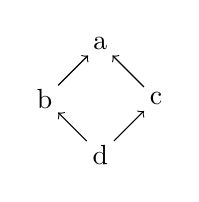
\begin{tikzpicture}[baseline=(current bounding box.center)]
            \node (top) at (0, 0) {a};
            \node[below left of = top] (left) {b};
            \node[below right of = top] (right) {c};
            \node[below right of = left] (bottom) {d};
            \draw[->, shorten <=-2pt, shorten >=-2pt,] (left) -- (top);
            \draw[->, shorten <=-2pt, shorten >=-2pt,] (right) -- (top);
            \draw[->, shorten <=-2pt, shorten >=-2pt,] (bottom) -- (left);
            \draw[->, shorten <=-2pt, shorten >=-2pt,] (bottom) -- (right);
        \end{tikzpicture}
        \xrightarrow{\varphi}
        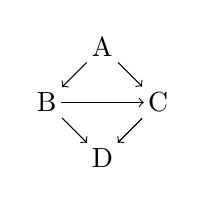
\begin{tikzpicture}[baseline=(current bounding box.center)]
            \node (top) at (0, 0) {A};
            \node[below left of = top] (left) {B};
            \node[below right of = top] (right) {C};
            \node[below right of = left] (bottom) {D};
            \draw[->, shorten <=-2pt, shorten >=-2pt,] (top) -- (left);
            \draw[->, shorten <=-2pt, shorten >=-2pt,] (top) -- (right);
            \draw[->, shorten <=-2pt, shorten >=-2pt,] (left) -- (bottom);
            \draw[->, shorten <=-2pt, shorten >=-2pt,] (right) -- (bottom);
            \draw[->, shorten <=-2pt, shorten >=-2pt,] (left) -- (right);
        \end{tikzpicture}
    \]
    If \(\varphi^{-1}\) were order-reversing, then \(X \leq Y\) would imply that \(\varphi^{-1}(X) \geq \varphi^{-1}(Y)\), for any \(X\) and \(Y\) in the second lattice. But while we have \(B \leq C\), their preimages \(\varphi^{-1}(B) = b\) and \(\varphi^{-1}(C) = c\) are in no relation in the first lattice.

    \item Let \(a, b \in \symcal{L}\). Let \(x \coloneq a \wedge b\). By the definition of the meet, we have that \(x \leq a\), \(x \leq b\) and for any \(c \in \symcal{L}\) with \(c \leq a\), \(c \leq b\) we must have \(c \leq x\).

    Since \(\varphi\) is order-reversing, we get that \(\varphi(x) \geq \varphi(a)\) and \(\varphi(x) \geq \varphi(b)\). For any \(c' \in \symcal{L}'\) with \(c' \geq \varphi(a)\) and \(c' \geq \varphi(b)\), we have that \(\varphi^{-1} (c') \leq \varphi^{-1}(\varphi(a)) = a\) and \(\varphi^{-1} (c') \leq \varphi^{-1}(\varphi(b)) = b\). Hence, since \(x\) is the meet of \(a\) and \(b\), we can deduce that \(\varphi^{-1} (c') \leq x\). Applying \(\varphi\) gives us \(\varphi(\varphi^{-1}(c')) = c' \leq \varphi(x)\), proving that \(\varphi(x) = \varphi(a \wedge b)\) is the join of \(\varphi(a)\) and \(\varphi(b)\), i.e. \(\varphi(a \wedge b) = \varphi(a) \vee \varphi(b)\).
\end{enumerate}
\end{solution}

\begin{exercise}
Let \(G\) be a group and \(E\) a field. A \emph{linear character} of \(G\) in \(E\) is a group homomorphism \(\sigma \colon G \to \symrm{GL}_1 (E)\).

Show that every set \(\Set{ \sigma_1, \dots, \sigma_n }\) of distinct linear characters of a group \(G\) in a field \(E\) is independent: if \(\sum_{i=1}^{n} x_i \sigma_i(g) = 0\) for all \(g \in G\), then \(x_i = 0\), \(\forall i = \overline{1, n}\). (i.e. \(\Maps{G}{E}\) is an \(E\)-vector space and \(\Set{ \sigma_1, \dots, \sigma_n } \subset \Maps{G}{E}\) is linearly independent)
\end{exercise}
\begin{proof}
We will prove this by induction.

For \(n = 1\), it's clear: \(x_1 \sigma_1 (g) = 0\) for all \(g \in G\) implies that \(x_1 = 0\), since \(\sigma_1 (g)\) is a unit in \(E\).

Suppose now that we know the statement holds for \(k - 1\) and want to prove it for \(k\). Let \(\Set{ \sigma_1, \dots, \sigma_k }\) be a set of independent linear characters and \(\Set{ x_1, \dots, x_k } \subset E\) such that
\[
    x_1 \sigma_1 (g) + \dots + x_k \sigma_k (g) = 0
\]
for all \(g \in G\).

Fix an element \(h \in G\). Multiplying the above equation by \(\sigma_{k} (h)\) gives
\[
    x_1 \sigma_1 (g) \sigma_k (h) + \dots + x_k \sigma_k (g) \sigma_k (h) = 0
\]
while replacing \(g\) with \(g h\) in the first equation gives
\begin{gather*}
    x_1 \sigma_1 (g h) + \dots + x_k \sigma_k (g h) = 0 \\
    \iff x_1 \sigma_1 (g) \sigma_1 (h) + \dots + x_k \sigma_k (g) \sigma_k (h) = 0
\end{gather*}
for all \(g \in G\). Subtracting the two new equations, the last term cancels out and we're left with
\[
    x_1 \cdot (\sigma_1 (h) - \sigma_k (h)) \cdot \sigma_1 (g) + \dots + x_{k - 1} \cdot (\sigma_{k - 1} (h) - \sigma_k(h)) \cdot \sigma_{k - 1} (g) = 0
\]
which holds for all \(g \in G\). More concisely,
\[
    \sum_{i = 1}^{k - 1} \left(x_i \cdot (\sigma_i (h) - \sigma_k (h))\right) \cdot \sigma_i = 0
\]
This is a linear combination of \(k - 1\) characters, so we can apply the induction hypothesis to conclude that the coefficients \(x_i \cdot (\sigma_i (h) - \sigma_k(h)) = 0\), for all \(i = \overline{1, k - 1}\). In particular, since the characters are \emph{distinct}, for each index \(i\) we can find some \(h_i \in G\) for which \(\sigma_{i} (h_i) \neq \sigma_{k} (h_i)\), which shows that \(x_i\) must be zero.

Replacing \(x_1 = \dots = x_{k - 1} = 0\) in the original equation, we have
\[
    x_k \sigma_k (g) = 0
\]
for all \(g \in G\). By the base case of the induction, \(x_k\) is also zero. Hence, \(x_i = 0\) for all \(i = \overline{1, k}\), which is what we had to show.
\end{proof}

\begin{exercise}
Let \(p\) be a prime number and \(n \in \naturals^*\). For \(q \coloneq p^n\), show that the finite field \(\finitefield{q}\) has exactly one subfield of order \(p^d\) for every divisor \(d\) of \(n\), and no others.
\end{exercise}
\begin{proof}
In the previous homework, we have shown that \(\Gal{\finitefield{q}}{\finitefield{p}}\) is cyclic of order \(n\). We will denote this group by \(C_n\).

Using the Galois correspondence, the conclusion is equivalent to showing that \(C_n\) has exactly one subgroup of index \(d\). Letting \(e = n / d\), this is the same as showing that \(C_n\) has exactly one subgroup of order \(e\).

The basic theory of cyclic groups tells us that \(C_n\) is isomorphic to \(\left(\integersmod{n}, +\right)\). The subgroup generated by \(\widehat{d}\) is \(\Set{ \widehat{0}, \widehat{d}, 2 \widehat{d}, \dots, (e-1) \widehat{d} }\), which has order \(e\). Conversely, if \(\Set{ \widehat{0}, \widehat{x_1}, \dots, \widehat{x_{e - 1}} }\) is a subgroup of order \(e\), then we can write each element \(\widehat{x_j}\) as \(k_j \, \widehat{1}\). Furthermore, we have \(e \, \widehat{x_j} = \widehat{0}\) for any \(j\), since the order of any individual element must divide the order of the subgroup. Combining these two remarks shows us that \(e k_j \widehat{1} = \widehat{0}\), hence \(e \cdot k_j = n \cdot m\) for some \(m \in \naturals\). Writing \(n = d \cdot e\), we get that \(k_j = d \cdot m\), hence this subgroup is actually the one generated by \(\widehat{d}\).
\end{proof}


\end{document}
